  % !TEX encoding = UTF-8 Unicode
% $Header: /cvsroot/latex-beamer/latex-beamer/solutions/conference-talks/conference-ornate-20min.en.tex,v 1.6 2004/10/07 20:53:08 tantau Exp $

\documentclass[]{beamer}
\usepackage{icomma}
\usepackage{xltxtra}
\newfontfamily\DejaSans{DejaVu Sans}

% This file is a solution template for:

% - Talk at a conference/colloquium.
% - Talk length is about 20min.
% - Style is ornate.

\mode<presentation>
{
  \usetheme{Warsaw}
  % or ...

  %\setbeamercovered{transparent}
  % or whatever (possibly just delete it)
  
  \setbeamertemplate{navigation symbols}{}
  
  \newcommand*\oldmacro{}%
  \let\oldmacro\insertshorttitle%
  \renewcommand*\insertshorttitle{%
    \oldmacro\hfill%
    \insertframenumber\,/\,\inserttotalframenumber}
}

\usepackage[utf8]{inputenc}
% or whatever

\usepackage{times}
\usepackage{multirow}
\usepackage[T1]{fontenc}
\usepackage{graphicx}
\usepackage{eso-pic}
\usepackage{color}
\usepackage{tikz}
\usepackage{wasysym}
\usepackage{eurosym}

% Or whatever. Note that the encoding and the font should match. If T1
% does not look nice, try deleting the line with the fontenc.

\title[]
{Mangaki, an open source anime/manga recommender system, in Python}

\author[]
{Jill-Jênn Vie}

\institute[]
{
\includegraphics[width=0.42\linewidth]{figures/mangaki.png}}

\date
{HN Kansai, Kobe -- 2(/01)7/2017}

\begin{document}

\definecolor{vert}{rgb}{0.07 0.54 0.07}

{
\setbeamertemplate{headline}[default]
\begin{frame}
	\titlepage
\end{frame}
}

\def\R{\mathcal{R}}
\def\N{N}
\newcommand\good{{\color{green!50!black}\DejaSans ☺}}
\newcommand\neutral{{\color{blue}\DejaSans 😐}}
\newcommand\bad{{\color{red}\DejaSans ☹}}

\begin{frame}
  \frametitle{Outline}
  \begin{itemize}
    \item[1.] Who I am
    \item[2.] Mangaki ($\simeq$ Netflix? or Movielens?)
    \item[3.] Some interesting problems
    \item[4.] Demo!
  \end{itemize}
\end{frame}

\begin{frame}
  \frametitle{Hi, I'm JJ}
  \begin{itemize}
    \item Fresh out of school
    \item Next April, researcher at RIKEN AI, Tokyo
    \item Supervised by Hisashi Kashima, in Kyoto University
    \item Super-supervised by my girlfriend, in Nara
  \end{itemize}
  \uncover<2>{\centering
  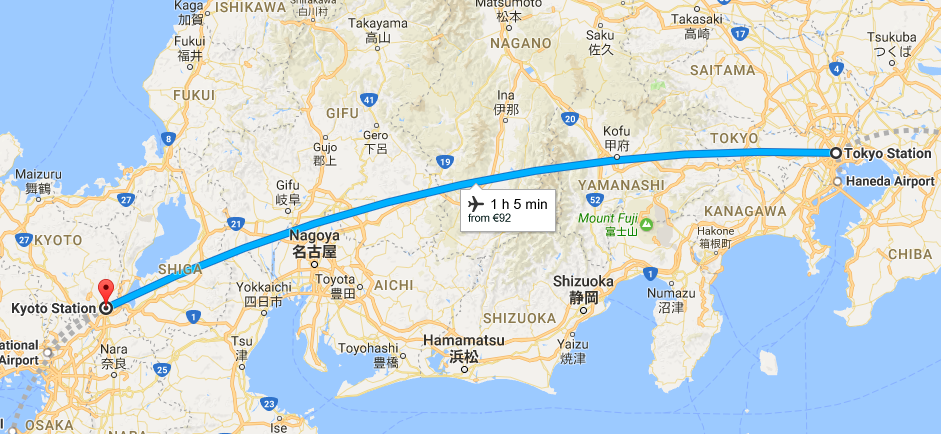
\includegraphics[width=\linewidth]{figures/flights.png}\\
  (If you can get cheap fares, I'm interested.)}
\end{frame}

\begin{frame}
  \frametitle{Let's make the Netflix of manga}
  Because France is the 2\textsuperscript{nd} manga consumer in the world

  \begin{itemize}
    \item[1.] Japan - 500M volumes
    \item[2.] France - 13M volumes \only<2->{(actually, \alert{2\%})}
    \item[3.] US - 9M volumes
  \end{itemize}

  \begin{exampleblock}{Japan Expo, summer festival about Japanese culture}
  \begin{itemize}
  \item manga / anime / sh\= ogi / washoku / ikebana / shiatsu
  \item During Tanabata
  \item 250,000 tickets over 4 days
  \end{itemize}
  \vspace{-2mm}
  \end{exampleblock}
  \vspace{2mm}
  \uncover<3>{\centering \huge (Don't forget the video.)\\
  \footnotesize You always forget the video.}
\end{frame}

\newcommand\discrete[1]{\textcolor{gray}{\hfill {\em \small #1}}}

\begin{frame}
  \frametitle{Mangaki}
    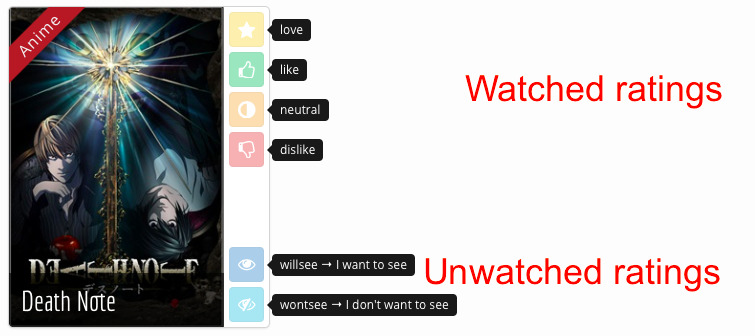
\includegraphics[width=\textwidth]{figures/ratings.jpg}
  \begin{itemize}
  \item 2100 users
  \item 15000 works \discrete{anime / manga / OST}
  \item 310000 ratings \discrete{fav / like / dislike / neutral / willsee / wontsee}
  \item People rate a few works \discrete{Preference Elicitation}
  \item And receive recommendations \discrete{Collaborative Filtering}
  \end{itemize}
\end{frame}

\begin{frame}
  \frametitle{Our Team}
  \begin{columns}
  \begin{column}{0.5\textwidth}
    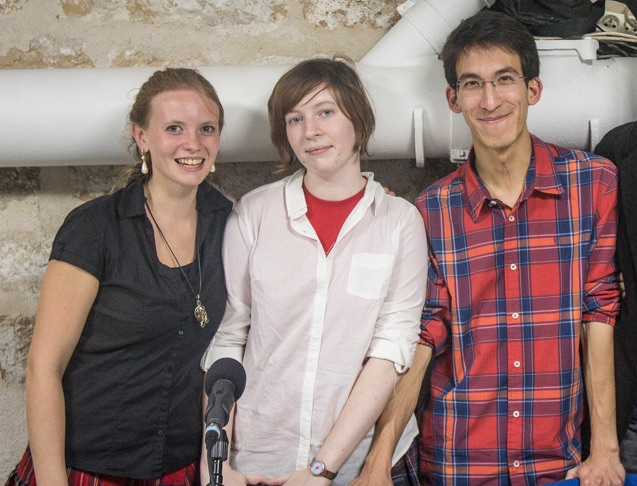
\includegraphics[width=\textwidth]{figures/trio.jpg}
  \end{column}
  \begin{column}{0.5\textwidth}
    {\em Let's use algorithms to discover pearls of Japanese culture!}\\[5mm]
    26 members, including:\\\hspace{7mm} 3 mad developers\\\hspace{14mm} 1 graphic designer
  \end{column}
  \end{columns}
  \vspace{2mm}
  \begin{itemize}
  \item 2014 -- \alert{Mangaki}
  \item 2015 -- Prize: Microsoft Ventures (Student Demo Cup)
  \item 2016 -- Prize: Japanese Cultural Institute in Paris\\[1mm]\pause\hfill\small\em We flew to Tokyo and met Cool Japan Fund!
  \end{itemize}
\end{frame}

\begin{frame}
  \frametitle{Mangaki = Movielens of manga}
  \centering
  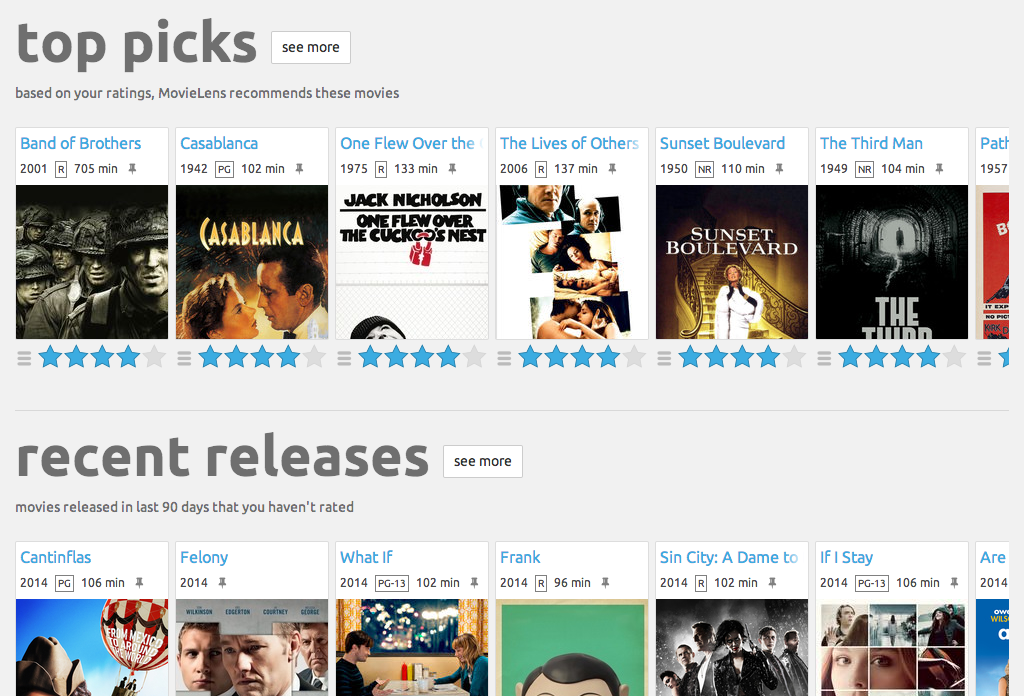
\includegraphics[width=\textwidth]{figures/movielens.png}\\
  Data is freely available for research and benchmarks
\end{frame}

\begin{frame}
	\frametitle{Collaborative Filtering}
	\begin{block}{Problem}
		\begin{itemize}
		\item Every user rates some items (1\%)
    \item How to guess the missing ratings?
		\end{itemize}
    \vspace{-2mm}
	\end{block}
  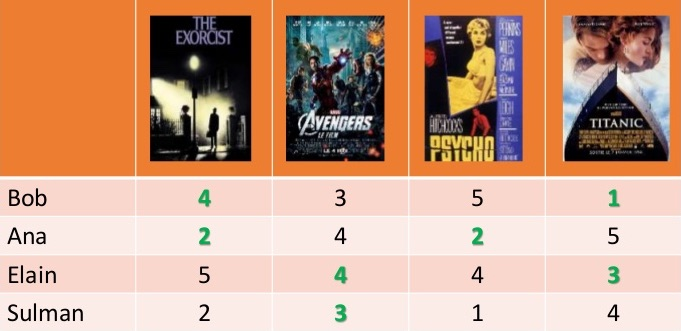
\includegraphics[width=\linewidth]{figures/cf.jpg}
\end{frame}

\begin{frame}
  \frametitle{Preference Elicitation}
  \begin{block}{Problem}
      What questions to ask adaptively to a new user?
  \end{block}
  \centering
  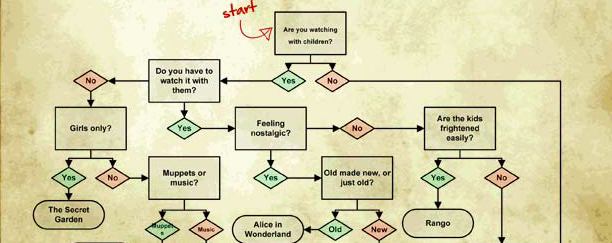
\includegraphics[width=\linewidth]{figures/flowchart.png}\\
  \em What to Watch on Netflix, Silver Oak Casino, 2013
\end{frame}

\begin{frame}
  \frametitle{Actually, Yahoo Labs did that research too}
  \centering
  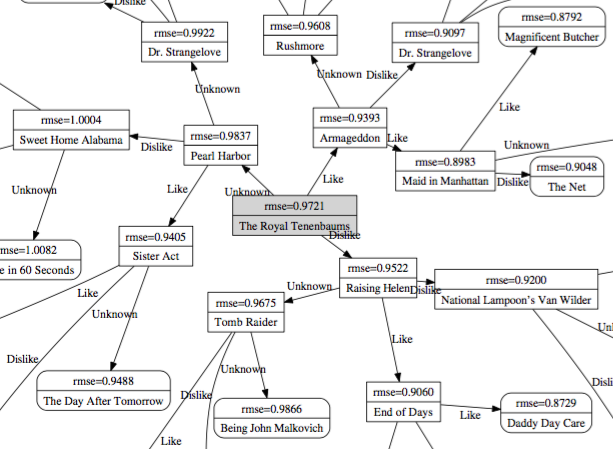
\includegraphics[width=0.9\linewidth]{figures/decisiontree.png}\\
  Good balance between like, dislike and unknown outcomes.
\end{frame}

\begin{frame}[fragile]
	\frametitle{Our anonymized data}
  \begin{verbatim}
user_id,work_id,rating
634,4319,wontsee
1380,6386,willsee
1683,3512,wontsee
1228,6777,like
143,2185,like
816,2805,wontsee
697,6356,wontsee
186,1383,neutral
1666,686,willsee
755,3802,neutral
...
  \end{verbatim}
  \vspace{-7mm}
  (310,000 lines)\bigskip

  Let's do some principal components analysis.
\end{frame}

\begin{frame}
  \frametitle{user2vec: plotting every user on a map}
  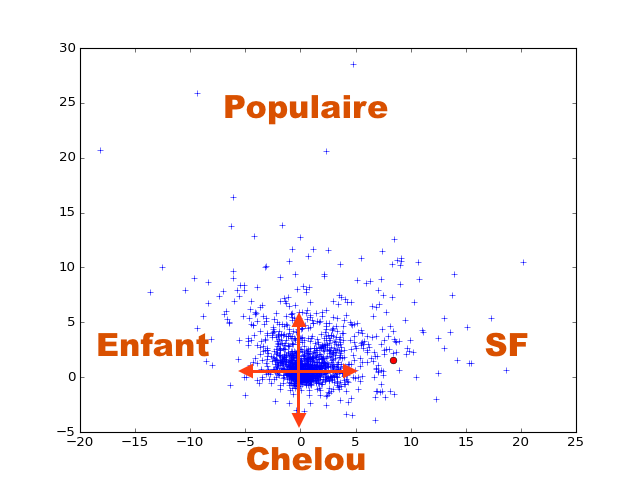
\includegraphics[width=\linewidth]{figures/map.png}
\end{frame}

\begin{frame}
  \frametitle{user2vec: plotting every user on a map}
  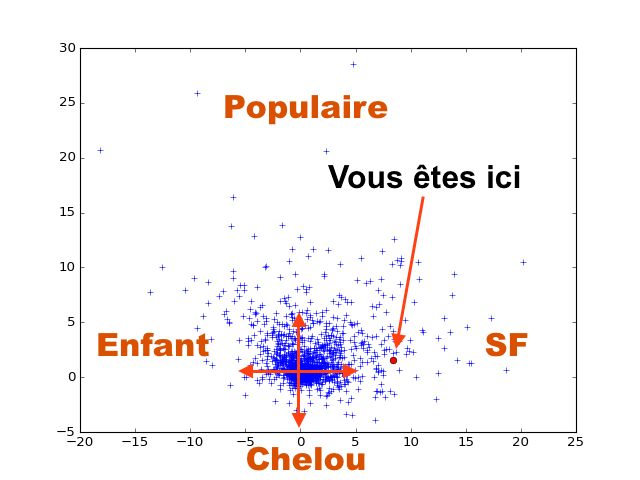
\includegraphics[width=\linewidth]{figures/here.png}
\end{frame}

\begin{frame}
    \frametitle{Mangaki's Explained Profiles}
    \begin{block}{$P_1$ loves Ghibli and cyberpunk, hates teen stories}
    \begin{itemize}
    \item[\good] \emph{Princess Mononoké}, \emph{Spirited Away} (Chihiro)
    \item[\good] \emph{Cowboy Bebop}, space opera similar to \emph{Firefly}
    \item[\good] \emph{Paprika}, which inspired \emph{Inception}
    \item[\bad] \emph{Naruto}, \emph{Bleach}
    \end{itemize}
    \end{block}
    \pause
    \begin{block}{$P_2$ loves really weird works, hates the most popular works}
    \begin{itemize}
    \item[\good] Erotic stories
    \item[\good] Same-family homosexual romances:\\\emph{Kiss x Sis}, \emph{Papa to Kiss in the Dark}
    \item[\bad] \emph{Attack on Titan}, \emph{Death Note}
    \end{itemize}
    \end{block}
\end{frame}

\begin{frame}
  \frametitle{What questions should be asked?}
  \centering
  points that are \alert{far from each other}\\
  =\\
  \alert{diverse} movies\bigskip

  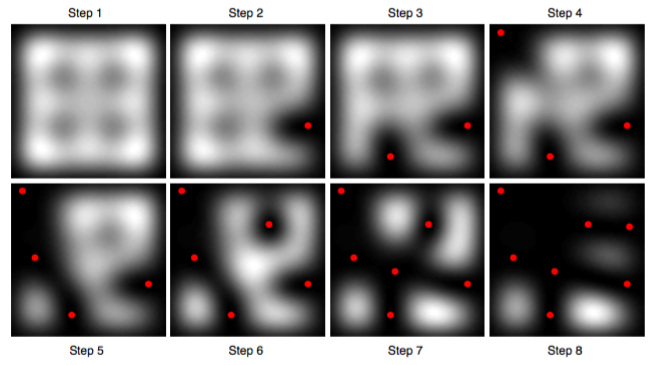
\includegraphics[width=\linewidth]{figures/dpp.png}
\end{frame}

\begin{frame}
  \frametitle{Preference elicitation: sampling a diverse subset}
  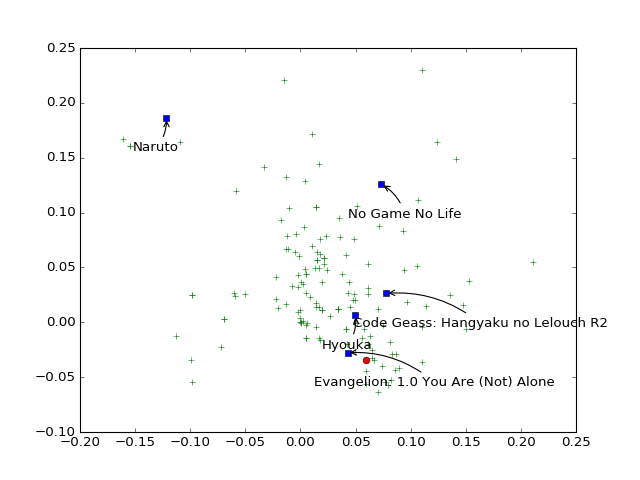
\includegraphics[width=\linewidth]{figures/1.png}
\end{frame}

\begin{frame}
  \frametitle{Summing up}
  \begin{itemize}
    \item Mangaki is a \alert{non-profit} recommender system\\
    \hfill (discover precious pearls of Japanese animation)\\[1cm]
    \item Mangaki data is a \alert{nice playground for trying algorithms}\\
    \hfill (so far, \texttt{numpy}, \texttt{scikit-learn}, \texttt{tensorflow})\\[1cm]
    \item Maybe we could make a service for general content?\\
    \hfill (like Algolia or ElasticSearch)
  \end{itemize}
  \centering
  \uncover<2>{\huge Time for demo?}
\end{frame}

\begin{frame}
	\frametitle{Thanks for listening!}
  \centering
  \LARGE
	
\includegraphics[width=1cm]{figures/twitter.png}\,\,\raisebox{1.5mm}{@jjvie}
  \vspace{5mm}
  
\includegraphics[width=\linewidth]{figures/mangaki.png}\\
  mangaki.fr \hfill Also on GitHub!
\end{frame}

\end{document}
